\chapter{Cas d'utilisation}

\section{Diagramme}

\begin{figure}
  \centering
  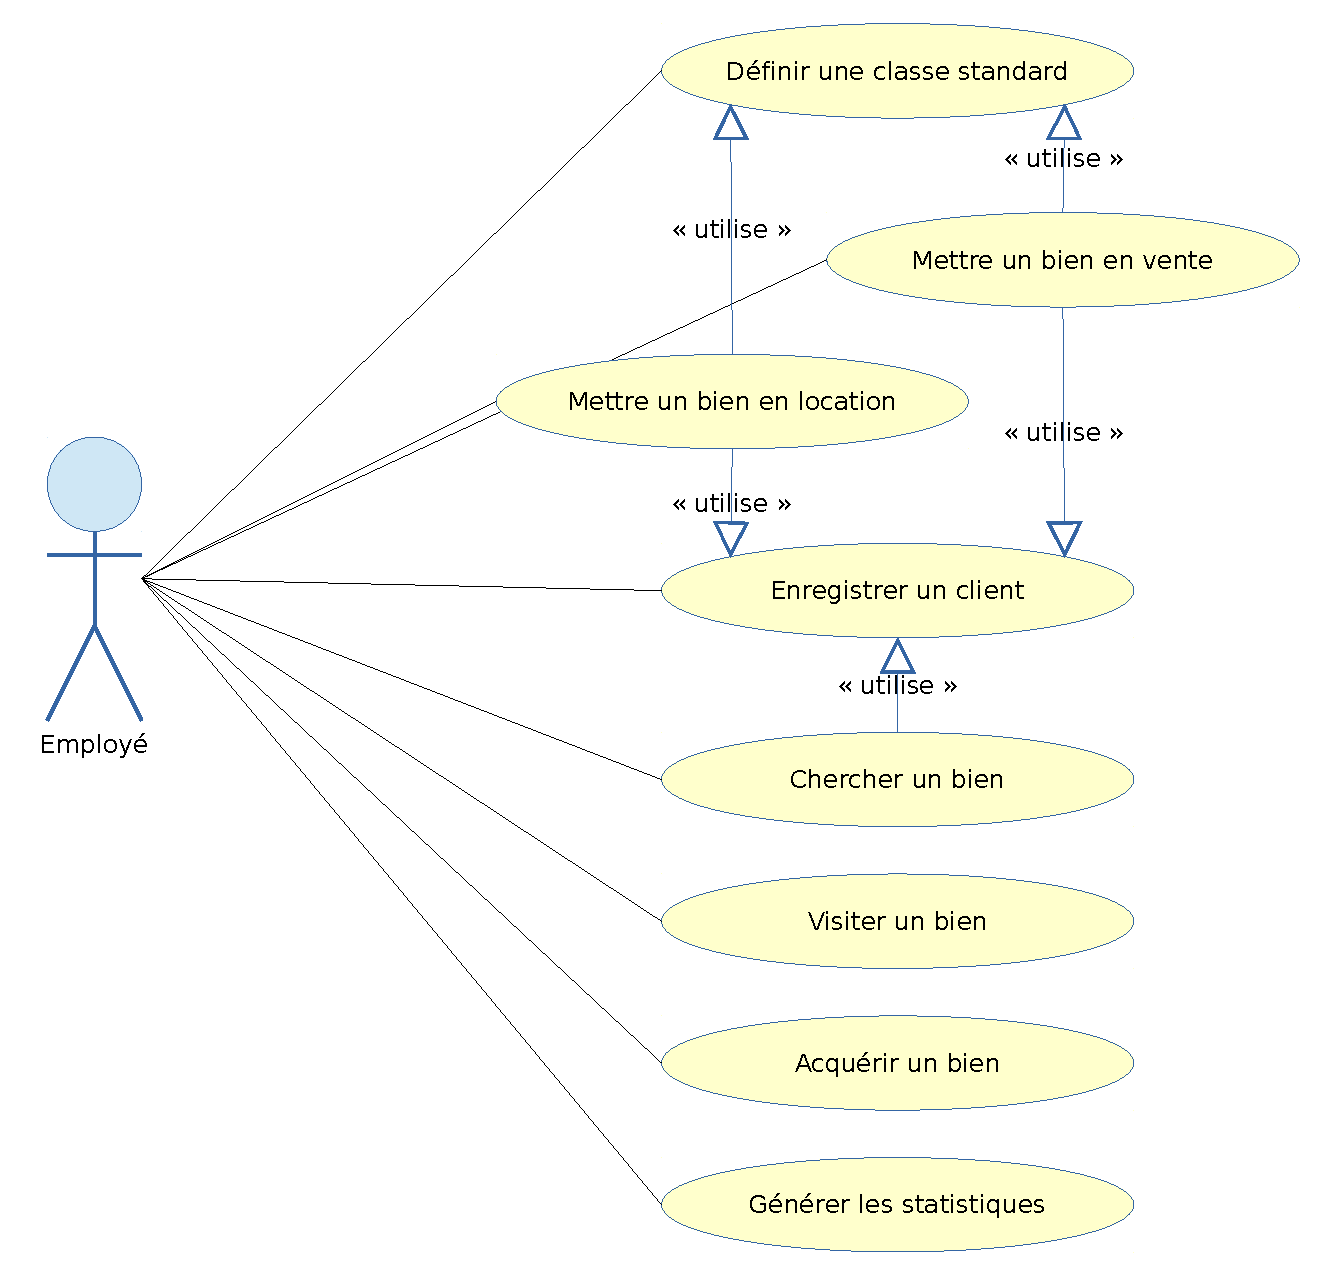
\includegraphics[width=0.95\textwidth]{IMG/uc}
  \caption{Cas d'utilisation}
  \label{img_uc}
\end{figure}

La figure \refpage{img_uc} illustre les cas d'utilisation du projet.

\section{Scénarios}

\subsection{Définir une classe standard}

L'employé crée une nouvelle classe standard et y enregistre les paramètres que les biens devront remplir pour en faire partie.

\subsection{Proposer un bien}

Le bien à mettre en vente ou en location doit appartenir à un client enregistré dans le système. S'il s'agit d'un nouveau client, ce dernier sera d'abord enregistré. L'employé va enregistrer les différents paramètres du bien dans le système. Les paramètres à enregistrer dépendront du type de bien et du type d'offre (voir tableau \refpage{tbl_usage_attribut_bien_immobilie}). Le bien se verra attribuer une classe standard d'après ses paramètres. Si aucune classe standard n'existe pour ce bien, il faudra en créer une.

\subsection{Enregistrer un client}

L'employé va enregistrer les données du client dans le système. Les données à enregistrer sont le nom, l'adresse et le numéro de téléphone. S'il s'agit d'un offrant, l'employé enregistrera également le téléphone professionnel ainsi que les heures heures auxquelles le client est accessible sur chaque numéro. Sinon, le client sera associé à une série de classes standards qui correspondent aux types de biens qu'il recherche.

\subsection{Enregistrer une demande}

L'enregistrement d'une demande d'un bien sera effectuée pour un client enregistré dans le système. S'il s'agit d'un nouveau client, ce dernier sera d'abord enregistré. Le client sera associé à une série de classes standard correspondant aux critères qu'il a donné. Le système va générer la liste de tous les biens correspondants à ces classes standard et encore disponibles. Cette liste reprend la localisation du bien, le prix demandé et les informations relatives à la superficie. Le résultat sera imprimé et soumis au client.

Le client pourra examiner la liste et éliminer de suite les biens immobiliers qui ne l'intéresse pas.

\subsection{Organiser une visite de biens}
\label{section_UC_organiser_une_visite_de_biens}

Ce cas d'utilisation va permettre de convenir de rendez-vous pour la visite de biens immobiliers. Ces visites concernent un client qui doit être actif dans le système. Si ce n'est pas le cas, il faudra activer ce client.

Pour chacun des biens retenu par le client, un employé consulte, à l'aide d'un terminal, les informations s'y rapportant afin de fournir des renseignements plus précis tandis que son collègue recherche la photo correspondant dans le fichier. Grâce aux renseignements supplémentaires et à la photo, le client peut se faire une opinion sur le bien. L'employé enregistre alors l'accord ou le désaccord du client.

La terminaison de la consultation de tous les biens déclenche automatiquement, pour chaque bien retenu, l'affichage des dates et heures de visites déjà planifiées pour les autres clients intéressés par ce bien. En fonction de ces informations l'employé et le client conviennent ensemble d'une date et d'une heure de visite que l'employé enregistre. Il enregistre également le nom de la personne responsable de cette visite.

\subsection{Acquérir un bien}

Lorsqu'un client est intéressé par un bien, une proposition sera envoyée au propriétaire. Si ce dernier l'accepte, un contrat sera émis entre le propriétaire et l'acquéreur via l'agence.

Il est possible que le propriétaire n'accepte pas l'offre de l'acquéreur. Ce refus peut être définitif, ou déboucher sur une négociation qui aboutira à l'acceptation ou non d'une offre.

\subsection{Générer les statistiques}

De manière à fournir régulièrement des informations pertinentes au service de prospection, le service d'enregistrement des demandes produit un document statistique récapitulant les différents types de demandes. Cet état statistique est généré en fin de semaine ou dès que 100 demandes sont enregistrées. Ces statistiques seront mise à disposition des employés du service de prospection.

\section{Rapport}

J'ai commencé par ce diagramme afin d'avoir une idée générale des actions que l'application devra pouvoir réaliser. Il est basé sur la description des tâches à réaliser de l'énoncé.

Nous pourrions également envisager différents cas d'utilisation supplémentaires pour l'administration du système comme la modification des informations du système (mise à jour et suppression des classes standard, des biens, des clients, etc.), la gestion des accès des employés, la gestion des contrats, etc. Cette étude ne tiendrait toutefois pas dans ce document et je ne l'ai donc pas prise en compte.